% Author: Jan Schaumann <jschauma@netmeister.org>
% $Id: slides.tex,v 1.10 2005/04/04 21:42:02 jschauma Exp $
\special{! TeXDict begin /landplus90{true}store end }

% https://www.dns-oarc.net/oarc/services/porttest

\documentclass[xga]{xdvislides}
\usepackage[landscape]{geometry}
\usepackage{graphics}
\usepackage{graphicx}
\usepackage{colordvi}

\begin{document}
\setfontphv

\lhead{\slidetitle}                               % default:\lhead{\slidetitle}
\chead{CS615 - Aspects of System Administration}% default:\chead{\relax}
\rhead{Slide \thepage}                       % default:\rhead{\sectiontitle}
\lfoot{\Gray{DNS}}% default:\lfoot{\slideauthor}
\cfoot{\relax}                               % default:\cfoot{\relax}
\rfoot{\Gray{\today}}

\vspace*{\fill}
\begin{center}
	\Hugesize
		CS615 - Aspects of System Administration\\ [1em]
		DNS\\ [1em]
	\hspace*{5mm}\blueline\\ [1em]
	\Normalsize
		Department of Computer Science\\
		Stevens Institute of Technology\\
		Jan Schaumann\\
		\verb+jschauma@stevens.edu+ \\
		\verb+http://www.cs.stevens.edu/~jschauma/615/+
\end{center}
\vspace*{\fill}

\subsection{In the beginning...}
\vspace*{\fill}
\begin{center}
	\includegraphics[scale=0.8]{pics/2computers.eps} \\
\end{center}
\vspace*{\fill}

\subsection{In the beginning...}
\vspace*{\fill}
\begin{center}
	\includegraphics[scale=0.8]{pics/2computers-nic.eps} \\
\end{center}
\vspace*{\fill}

\subsection{In the beginning...}
\vspace*{\fill}
\begin{center}
	\includegraphics[scale=0.8]{pics/3computers.eps} \\
\end{center}
\vspace*{\fill}

\subsection{In the beginning...}
\vspace*{\fill}
\begin{center}
	\includegraphics[scale=0.8]{pics/3computers-1.eps} \\
\end{center}
\vspace*{\fill}

\subsection{In the beginning...}
\vspace*{\fill}
\begin{center}
	\includegraphics[scale=0.8]{pics/3computers-2.eps} \\
\end{center}
\vspace*{\fill}

\subsection{In the beginning...}
\vspace*{\fill}
\begin{center}
	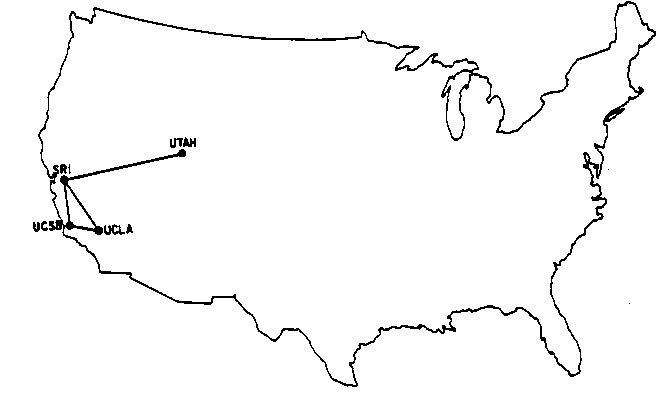
\includegraphics[scale=0.8]{pics/arpanet1.eps} \\
\end{center}
\vspace*{\fill}


\subsection{In the beginning...}
\begin{verbatim}
# Host Database
# This file should contain the addresses and aliases
# for local hosts that share this file.
#
127.0.0.1               localhost localhost.
#
# RFC 1918 specifies that these networks are "internal".
# 10.0.0.0      10.255.255.255
# 172.16.0.0    172.31.255.255
# 192.168.0.0   192.168.255.255
10.0.0.1	UCLA-TEST
10.0.0.2	SRI-SPRM
10.0.0.4	UTAH-CS
\end{verbatim}


\subsection{But then...}
\vspace*{\fill}
\begin{center}
	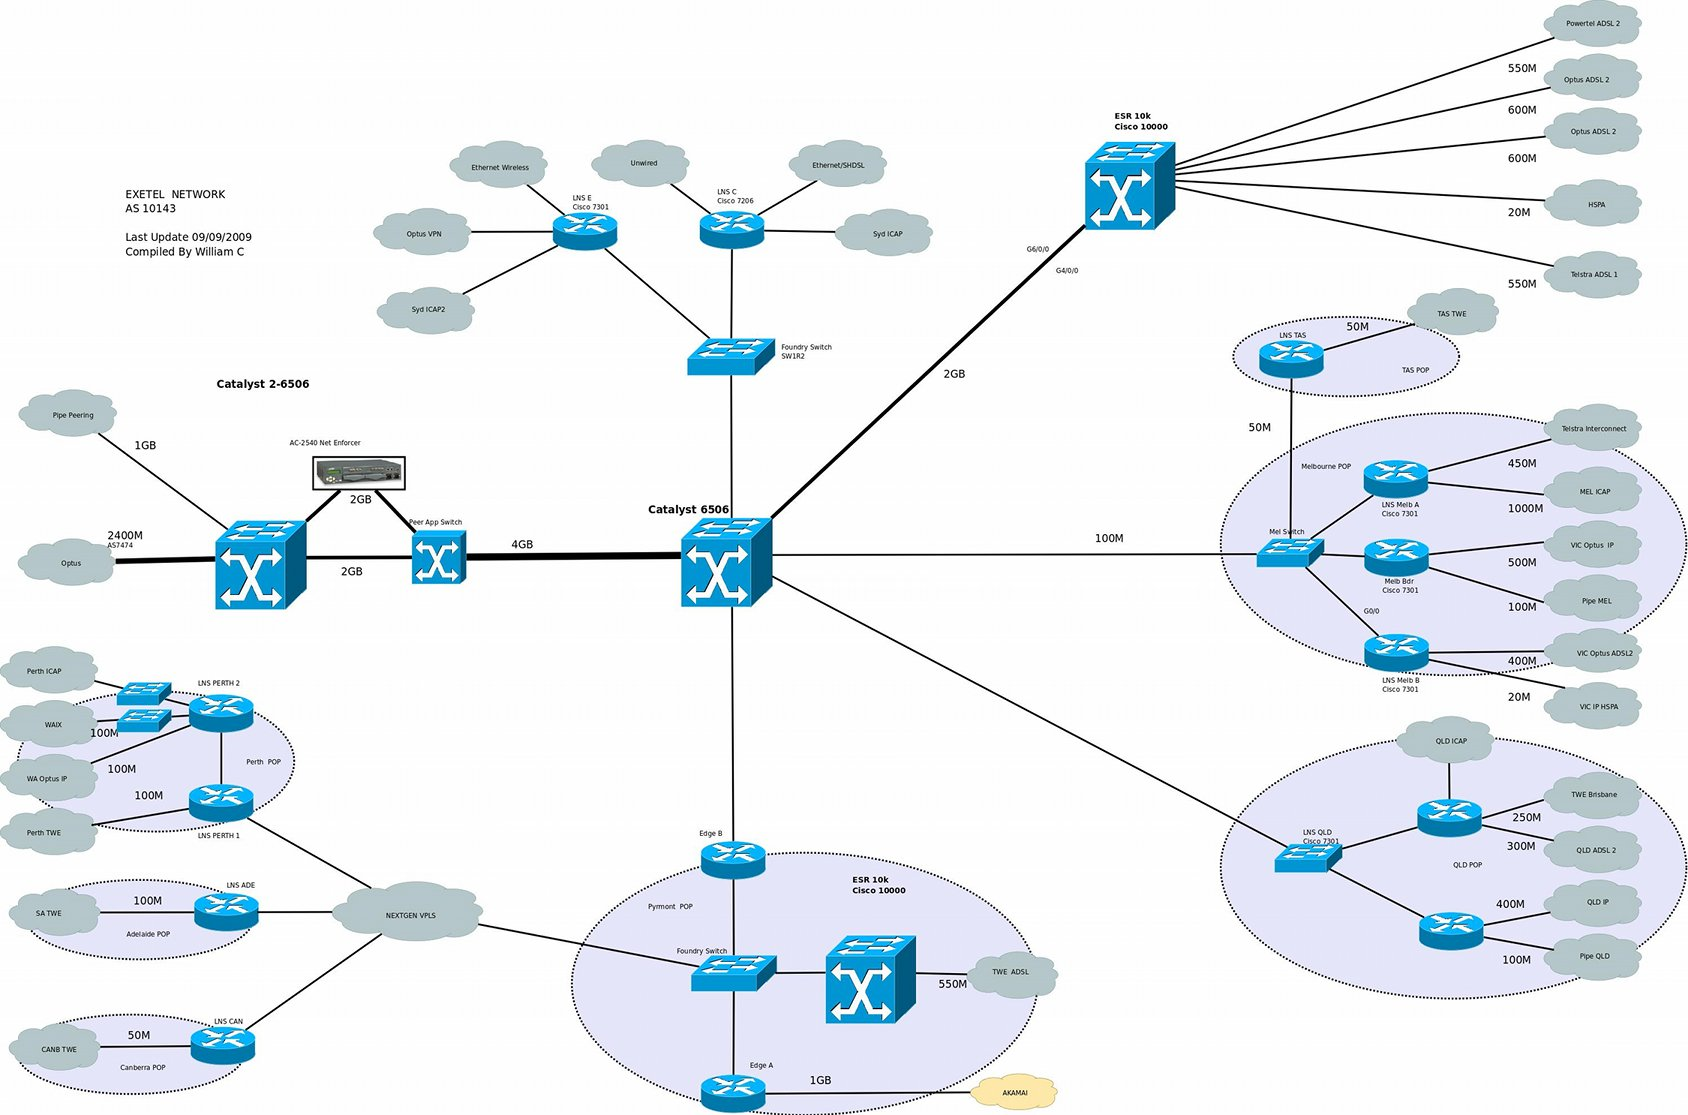
\includegraphics[scale=0.3]{pics/routed.eps} \\
\end{center}
\vspace*{\fill}

\subsection{The Domain Name System}
\vspace{.5in}
\begin{center}
	\Huge
	Computers like numbers. \\
\vspace{.5in}
\begin{verbatim}
         10011011111101100101100110011111
\end{verbatim}
\end{center}
\Normalsize

\subsection{The Domain Name System}
\vspace{.5in}
\begin{center}
	\Huge
	Computers like numbers. \\
\vspace{.5in}
\begin{verbatim}
      10011011  11110110  01011001  10011111

        155   .   246   .    89   .   159
\end{verbatim}
\end{center}
\Normalsize

\subsection{The Domain Name System}
\vspace{.5in}
\begin{center}
	\Huge
	People like names. \\
\vspace{.5in}
\verb+ash.cs.stevens-tech.edu+
\end{center}
\Normalsize


\subsection{The Domain Name System}
\vspace*{\fill}
\begin{center}
	
\includegraphics[scale=0.6]{pics/phonebook.eps}
\end{center}
\vspace*{\fill}

\subsection{The New Phonebook is here!}
\vspace*{\fill}
\begin{center}
	\verb+http://is.gd/XXp2sC+ \\
	\addvspace{.5in}
	\verb+wget -q -O - http://is.gd/XXp2sC | grep -c "^HOST"+
\end{center}
\vspace*{\fill}

\subsection{DNS: A distributed database}
\vspace*{\fill}
\begin{center}
	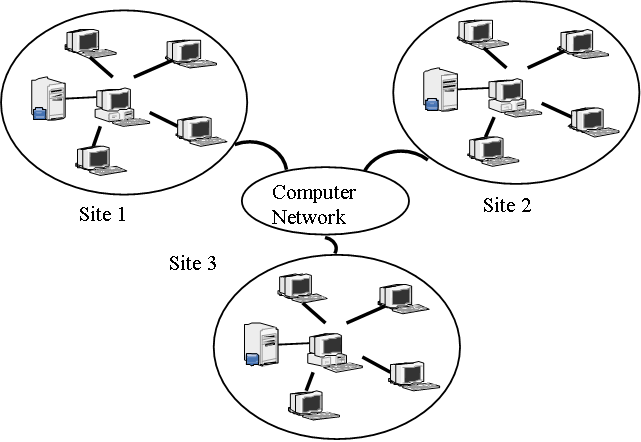
\includegraphics[scale=0.75]{pics/distributed-database.eps}
\end{center}
\vspace*{\fill}

\subsection{The Domain Name Space}
\vspace{.5in}
\begin{center}
	\Huge
	The domain name space consists of a tree of {\em domain} names.
\end{center}
\Normalsize

\subsection{DNS: A hierarchical system}
\vspace*{\fill}
\begin{center}
	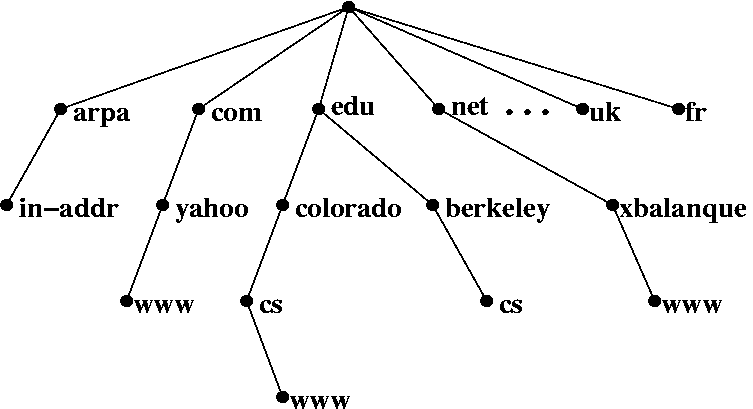
\includegraphics[scale=0.75]{pics/hierarchical-dns.eps}
\end{center}
\vspace*{\fill}

\subsection{The Domain Name Space}
\vspace{.5in}
\begin{center}
	\Huge
	The domain name space consists of a tree of {\em domain} names. \\
	\vspace{.5in}
	A subtree divides into {\em zones}.
\end{center}
\Normalsize

\subsection{The Domain Name Space}
\vspace{.5in}
\begin{center}
	\Huge
	The domain name space consists of a tree of {\em domain} names. \\
	\vspace{.5in}
	A subtree divides into {\em zones}. \\
	\vspace{.5in}
	Each node may contain {\em resource records}.
\end{center}
\Normalsize

\subsection{The Domain Name Space}
\vspace*{\fill}
\begin{center}
	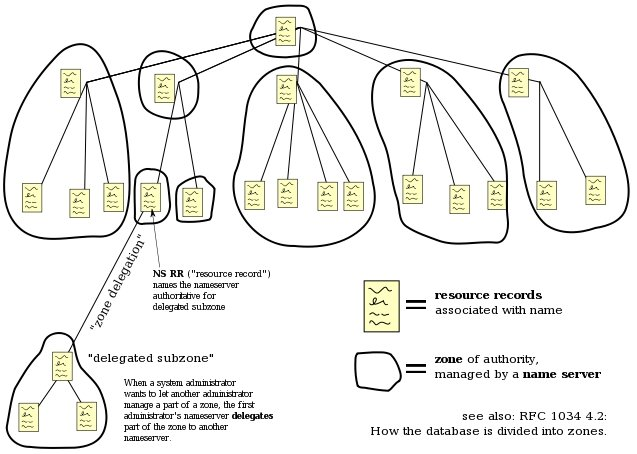
\includegraphics[scale=0.74]{pics/dns-space.eps}
\end{center}
\vspace*{\fill}

\subsection{Domain Names}
\vspace{.5in}
\begin{center}
	\Huge
	\verb+ash.cs.stevens-tech.edu+ \\
	\vspace{.5in}
	Domain Names are read from right to left and components separated by a ``\verb+.+''.
\end{center}
\Normalsize

\subsection{Domain Names}
\vspace{.5in}
\begin{center}
	\Huge
	\verb+ash.cs.stevens-tech.edu.+ \\
	\vspace{.5in}
	The {\em root} is known as ``\verb+.+'', but is usually left out.
\end{center}
\Normalsize

\subsection{Domain Names}
\vspace{.5in}
\begin{center}
	\Huge
	\verb+ash.cs.stevens-tech.+{\bf edu}\verb+.+ \\
	\vspace{.5in}
	There is a small number of {\em top level domains}.
\end{center}
\Normalsize

\subsection{Domain Names}
\vspace{.5in}
\begin{center}
	\Huge
	\verb+ash.cs.stevens-tech.+{\bf edu}\verb+.+ \\
	\vspace{.5in}
	There is a number of {\em top level domains}. \\
	\vspace{.5in}
	\Normalsize
	\begin{verbatim}
wget -O - ftp://rs.internic.net/domain/root.zone | \
        grep "IN<tab>*NS<tab>" | awk '{print $1}' | sort -u | wc -l
\end{verbatim}
	\vspace{.25in}
	\verb+http://data.iana.org/TLD/tlds-alpha-by-domain.txt+ \\
	\verb+https://en.wikipedia.org/wiki/List_of_Internet_top-level_domains+
\end{center}
\Normalsize


\subsection{Domain Names}
\vspace{.5in}
\begin{center}
	\Huge
	\verb+ash.cs.+{\bf stevens-tech}\verb+.edu.+ \\
	\vspace{.5in}
	Each {\em domain} can be divided into any number of {\em sub domains}.
\end{center}
\Normalsize

\subsection{Domain Names}
\vspace{.5in}
\begin{center}
	\Huge
	\verb+ash.+{\bf cs}\verb+.stevens-tech.edu.+ \\
	\vspace{.5in}
	Each {\em domain} can be divided into any number of {\em sub domains}.
\end{center}
\Normalsize

\subsection{Domain Names}
\vspace{.5in}
\begin{center}
	\Huge
	{\bf ash}\verb+.cs.stevens-tech.edu.+ \\
	\vspace{.5in}
	The left-most component of a domain name may be a {\em hostname}.
\end{center}
\Normalsize

\subsection{Fully Qualified Domain Names}
\vspace{.5in}
\begin{center}
	\Huge
	\verb+ash.cs.stevens-tech.edu.+ \\
	\vspace{.5in}
	A {\em hostname} with a domain name is known as a {\em FQDN}.
\end{center}
\Normalsize


\subsection{DNS servers come in two flavors}
\vspace*{\fill}
\begin{center}
	\begin{tabular}{ c c c }
	
\includegraphics[scale=1.5]{pics/vanilla.eps} & \hspace{.5in} & 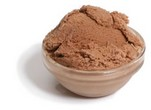
\includegraphics[scale=1.5]{pics/chocolate.eps} \\
	\hspace{.3in} \Huge Authoritative & & \hspace{.3in} \Huge Recursive \\
	\hspace{.3in} \Huge Nameservers & & \hspace{.3in} \Huge Nameservers \\
	\end{tabular}
\end{center}
\vspace*{\fill}

\subsection{Hostname resolution}
Resolution on a recursive nameserver (aka {\em resolver}) involves a number of queries:
\vspace{.5in}
\begin{verbatim}
$ nslookup ash.cs.stevens-tech.edu
Server:         127.0.0.1
Address:        127.0.0.1#53

Non-authoritative answer:
Name:   ash.cs.stevens-tech.edu
Address: 155.246.89.159

$
\end{verbatim}

\subsection{Hostname resolution}
Resolution on a {\em resolver} involves a number of queries:
\begin{verbatim}
18:39:27.186778 IP panix.netmeister.org.62105 > i.root-servers.net.domain:
        11585 [1au] A? ash.cs.stevens-tech.edu. (52)
18:39:27.446190 IP i.root-servers.net.domain > panix.netmeister.org.62105:
        11585- 0/8/8 (494)
18:39:27.446994 IP panix.netmeister.org.53168 > a.gtld-servers.net.domain:
        46575 [1au] A? ash.cs.stevens-tech.edu. (52)
18:39:27.481565 IP a.gtld-servers.net.domain > panix.netmeister.org.53168:
        46575- 0/6/3 (609)
18:39:27.481998 IP panix.netmeister.org.41071 > nrac.stevens-tech.edu.domain:
        24322 [1au] A? ash.cs.stevens-tech.edu. (52)
18:39:27.486035 IP nrac.stevens-tech.edu.domain > panix.netmeister.org.41071:
        24322*- 1/2/3 A[|domain]
\end{verbatim}
\Normalsize

\subsection{Hostname resolution}
Resolution on a {\em resolver} involves a number of queries:
\begin{verbatim}
$ host -t ns .
. name server I.ROOT-SERVERS.NET.
. name server D.ROOT-SERVERS.NET.
. name server C.ROOT-SERVERS.NET.
. name server M.ROOT-SERVERS.NET.
. name server F.ROOT-SERVERS.NET.
. name server A.ROOT-SERVERS.NET.
. name server E.ROOT-SERVERS.NET.
. name server L.ROOT-SERVERS.NET.
. name server H.ROOT-SERVERS.NET.
. name server J.ROOT-SERVERS.NET.
. name server B.ROOT-SERVERS.NET.
. name server G.ROOT-SERVERS.NET.
. name server K.ROOT-SERVERS.NET.
$
\end{verbatim}

\subsection{Hostname resolution}
Resolution on a {\em resolver} involves a number of queries:
\begin{verbatim}
$ dig -t ns edu.
[...]
;; ANSWER SECTION:
edu.                    172800  IN      NS      l.edu-servers.net.
edu.                    172800  IN      NS      f.edu-servers.net.
edu.                    172800  IN      NS      c.edu-servers.net.
edu.                    172800  IN      NS      g.edu-servers.net.
edu.                    172800  IN      NS      a.edu-servers.net.
edu.                    172800  IN      NS      d.edu-servers.net.

;; ADDITIONAL SECTION:
c.edu-servers.net.      36626   IN      A       192.26.92.30
d.edu-servers.net.      13274   IN      A       192.31.80.30
l.edu-servers.net.      36626   IN      A       192.41.162.30
[...]
$
\end{verbatim}
\Normalsize

\subsection{Hostname resolution}
Resolution on a {\em resolver} involves a number of queries:
\begin{verbatim}
$ dig @c.edu-servers.net -t ns stevens.edu.
[...]
;; AUTHORITY SECTION:
stevens.edu.            172800  IN      NS      nrac.stevens-tech.edu.
stevens.edu.            172800  IN      NS      sitult.stevens-tech.edu.

;; ADDITIONAL SECTION:
nrac.stevens-tech.edu.  172800  IN      A       155.246.1.21
sitult.stevens-tech.edu. 172800 IN      A       155.246.1.20
[...]
$
\end{verbatim}

\subsection{Hostname resolution}
\vspace*{\fill}
\begin{center}
	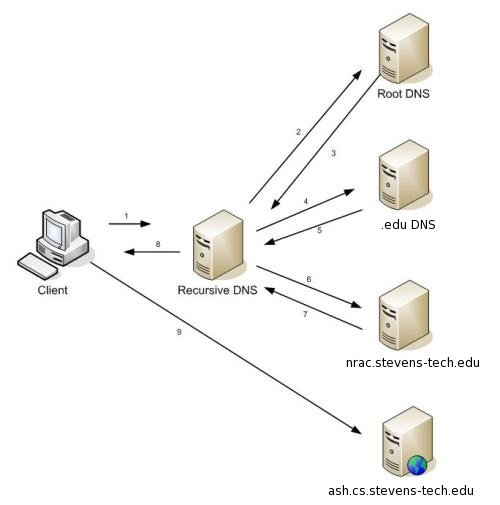
\includegraphics[scale=0.9]{pics/resolution.eps}
\end{center}
\vspace*{\fill}


\subsection{Hostname resolution}
Resolution on a {\em resolver} involves a number of queries:
\begin{verbatim}
$ nslookup ash.cs.stevens-tech.edu
Server:         127.0.0.1
Address:        127.0.0.1#53

Non-authoritative answer:
Name:   ash.cs.stevens-tech.edu
Address: 155.246.89.159

$
\end{verbatim}

\subsection{Hostname resolution}
\vspace*{\fill}
\begin{center}
	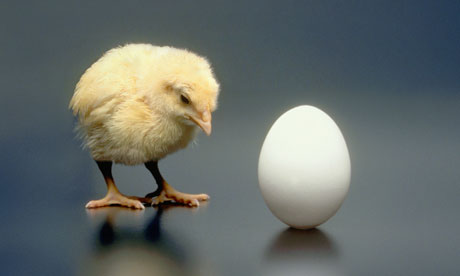
\includegraphics[scale=0.4]{pics/chicken-egg.eps} \\
	\vspace*{\fill}
\end{center}

\subsection{Hostname resolution}
\vspace*{\fill}
\begin{center}
	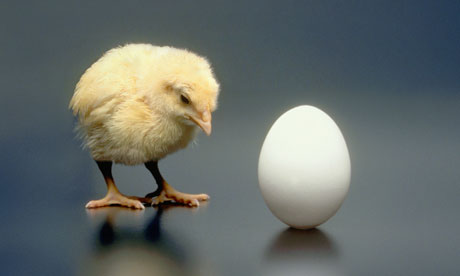
\includegraphics[scale=0.4]{pics/chicken-egg.eps} \\
	\addvspace{.2in}
	\verb+$ ftp -o - ftp.internic.net:/domain/db.cache | more+ \\
	\verb+http://www.internic.net/zones/named.root+
	\vspace*{\fill}
\end{center}

\subsection{Operation Global Blackout}
\vspace*{\fill}
\begin{center}
	
\includegraphics[scale=0.8]{pics/anonymous.eps} \\
	\addvspace{.2in}
	\verb+http://pastebin.com/XZ3EGsbc+ \\
	\addvspace{.1in}
\end{center}
\vspace*{\fill}

\subsection{DNS: A distributed system}
\vspace{.5in}
\begin{center}
	\Huge
	There are 13 \verb+root+ servers. \\
\end{center}
\Normalsize

\subsection{DNS: A distributed system}
\vspace{.5in}
\begin{center}
	\Huge
	There are 13 \verb+root+ servers. \\
	\vspace{.5in}
	Except... there are more.
\end{center}
\Normalsize

\subsection{DNS: A distributed system}
\vspace{.5in}
\begin{center}
	\Huge
	There are 13 \verb+root+ {\em authorities}. \\
\end{center}
\Normalsize

\subsection{DNS: A distributed system}
\vspace{.5in}
\begin{center}
	\Huge
	There are 13 \verb+root server+ {\em addresses}. \\
\end{center}
\Normalsize

\subsection{DNS: A distributed system}
\vspace{.5in}
\begin{center}
	\Huge
	There are hundreds of \verb+root+ servers. \\
\end{center}
\Normalsize

\subsection{DNS: A distributed system}
\vspace*{\fill}
\begin{center}
	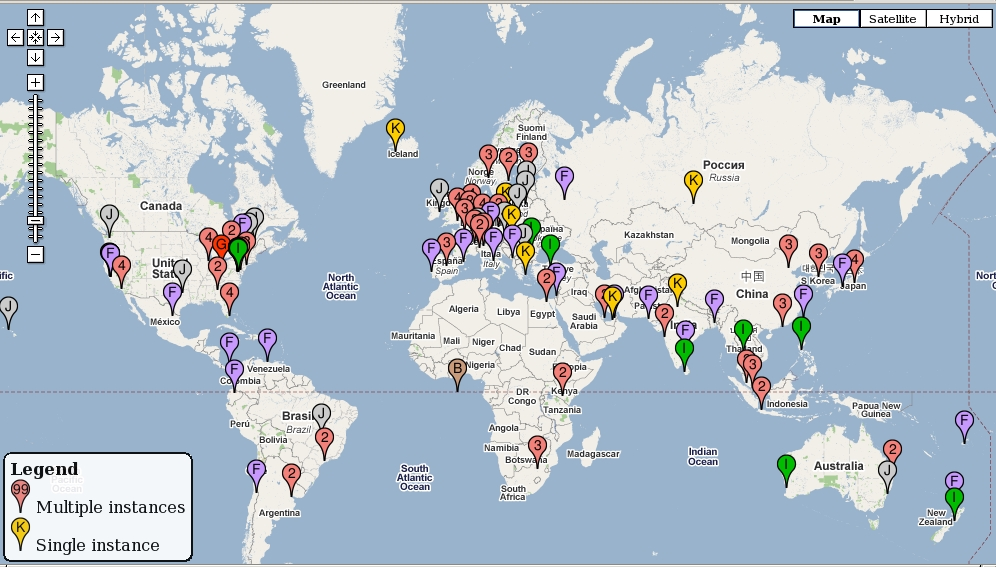
\includegraphics[scale=0.65]{pics/root-servers.eps}
\end{center}
\vspace*{\fill}

\subsection{Operation Global Blackout}
\vspace*{\fill}
\begin{center}
	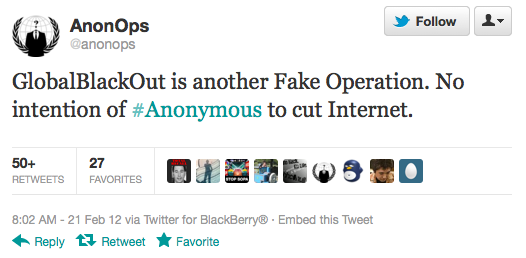
\includegraphics[scale=0.8]{pics/anonymous-tweet.eps} \\
\end{center}
\vspace*{\fill}

\subsection{DNS: A distributed database}
\vspace*{\fill}
\begin{center}
	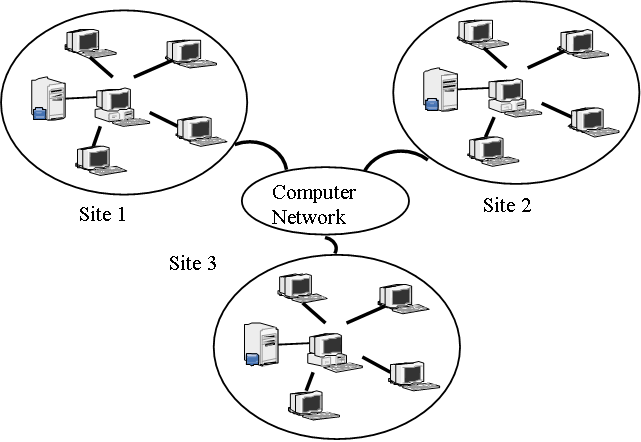
\includegraphics[scale=0.75]{pics/distributed-database.eps}
\end{center}
\vspace*{\fill}


\subsection{DNS Resource Records}
\begin{itemize}
	\item {\em NS} -- an authoritative name server
	\item {\em CNAME} -- the canonical name for an alias
	\item {\em SOA} -- marks the start of a zone of authority
	\item {\em PTR} -- a domain name pointer
	\item {\em HINFO} -- host information
	\item {\em MX} -- mail exchange
	\item {\em TXT} text strings
	\item ...
\end{itemize}

\subsection{DNS Resource Records}
\begin{verbatim}
$ host ash.cs.stevens-tech.edu
ash.cs.stevens-tech.edu has address 155.246.89.159
ash.cs.stevens-tech.edu mail is handled by 0 guinness.cs.stevens-tech.edu.
$
\end{verbatim}

\subsection{DNS Resource Records}
\begin{verbatim}
$ host a.gtld-servers.net
a.gtld-servers.net has address 192.5.6.30
a.gtld-servers.net has IPv6 address 2001:503:a83e::2:30
$ host -t ptr 2001:503:a83e::2:30
0.3.0.0.2.0.0.0.0.0.0.0.0.0.0.0.0.0.0.0.e.3.8.a.3.0.5.0.1.0.0.2.ip6.arpa
    domain name pointer a.gtld-servers.net.
$ host -t ptr 192.5.6.30
30.6.5.192.in-addr.arpa domain name pointer a.gtld-servers.net.
\end{verbatim}

\subsection{Creative uses of DNS Resource Records}
\begin{itemize}
	\item identifying sources of SPAM
	\item find out if the internet is on fire: \\
		\verb|dig +short txt istheinternetonfire.com|
	\item find ASN numbers by IP addresses: \\
		\verb|dig +short 159.89.246.155.origin.asn.cymru.com TXT|
	\item check a resolver's source port randomization (to help
		mitigate DNS Cache Poisoning attacks): \\
		\verb|dig +short porttest.dns-oarc.net TXT|
	\item using DNS to publish SSH key fingerprints (RFC4255,
ssh\_config(5) \verb+VerifyHostKeyDNS+; for best results combine with DNSSEC): \\
		\verb|dig +short ftp.netbsd.org SSHFP|
		\begin{verbatim}
ssh -o "VerifyHostKeyDNS yes" ftp.netbsd.org
[...]
Matching host key fingerprint found in DNS.
Are you sure you want to continue connecting (yes/no)?
\end{verbatim}
\end{itemize}

\newpage
\vspace*{\fill}
\begin{center}
    \Hugesize
        Hooray! \\ [1em]
    \hspace*{5mm}
    \blueline\\
    \hspace*{5mm}\\
        5 Minute Break
\end{center}
\vspace*{\fill}

%\subsection{HW4}
%\verb+http://www.cs.stevens.edu/~jschauma/615/s12-hw4.html+

\subsection{Reading}
DNS:
\begin{itemize}
	\item \verb+https://www.dns-oarc.net/oarc/services/porttest+
	\item \verb+http://www.kb.cert.org/vuls/id/800113+
	\item \verb+http://is.gd/XXp2sC+
	\item \verb+http://www.root-servers.org/+
	\item RFC 1034, 1035
\end{itemize}
\addvspace{.5in}

\end{document}
